\chapter{Генерация кода из описания модели}
\label{cha:code-gen}

\section{Выбор используемой нотации}
\label{sec:notation-choice}

В качестве нотации, используемой для задания модели, выбрано подмножество языка PROMELA,
описанного в \ref{sec:promela} и используемого верификатором SPIN. Это позволяет
использовать модели, созданные для SPIN, с минимальными изменениями. 

Следующие возможности PROMELA не реализованы:

\begin{enumerate}
\item Возможность создания новых процессов (т.е. все процессы должны быть активны изначально);
\item пользовательские типы данных (структуры и перечисления);
\item синхронные каналы (т.е. каналы нулевого размера, которые представляют собой <<точки
  рандеву>> между двумя процессами); поддерживаются асинхронные каналы ненулевого размера
  (за один переход возможна только одна операция с таким каналом -- запись одним процессом
  либо чтение другим);
\item возможность обращаться к явным и скрытым (IP) переменным других процессов.
\end{enumerate}

\section{Схема процесса генерации состояний}
\label{sec:idef0-codegen}

Основное время при генерации состояний уходит на составление множества $Next(s)$ для
текущего состояний $s$. Оно заключается в вычислении условий выполнимости текущих
инструкций всех процессов, присутствующих в $s$ (отсюда мы получаем множество
незаблокированных процессов $P_{ready}(s)$), после чего для каждого процесса $P$ из
$P_{ready}(s)$ генерируется новое состояние, получающееся в результате выполнения его
текущей инструкции (номер которой хранится в $IP_P$).

Для достижения большей производительности генерация состояний осуществляется кодом на
языке~C, который, в свою очередь, генерируется из описания модели.

Процесс генерации состояний изображен на рис.~\ref{fig:idef0-codegen}. Исходное описание
модели считывается парсером и переводится во внутреннее представление в виде графа команд
и условий их выполнимости. 

% \begin{figure}[ht]
%   \centering
%   \begin{tikzpicture}[->,>=stealth',node distance=2cm]
%     \tikzstyle{state} = [circle,fill=none,draw=black,thick,text=black]
%     \tikzstyle{trans} = [rectangle split,rectangle split parts=2,rounded corners,thick,fill=none,draw=black,text=black]
%     \tikzstyle{line}  = [draw, -latex']

%     \node[state]     (S0)                     {$s_0$};
%     \node[trans]     (T0) [below       of=S0] {
%       \begin{tabular}{l}
%         \scriptsize$lfork = 0$
%         \nodepart{second}
%         \scriptsize$lfork \leftarrow 1$
%       \end{tabular}
%     };
%     \node[state]     (S1) [below       of=T0] {$s_1$};
%     \node[trans]     (T1) [below left  of=S1] {
%       \begin{tabular}{l}
%         \scriptsize$rfork = 0$
%         \nodepart{second}
%         \scriptsize$rfork \leftarrow 1$
%       \end{tabular}
%     };
%     \node[state]     (S2) [below       of=T1] {$s_2$};
%     \node[trans]     (T2) [below right of=S1] {
%       \begin{tabular}{l}
%         \scriptsize$rfork \neq 0$
%         \nodepart{second}
%         \scriptsize$lfork \leftarrow 1$
%       \end{tabular}
%     };
%     \node[state]     (S3) [below       of=T2] {$s_3$};
%     \node[trans]     (T3) [below       of=S2] {
%       \begin{tabular}{l}
%         \nodepart{second}
%         \scriptsize$n_{eat} = n_{eat} + 1$
%       \end{tabular}
%     };
%     \node[state]     (S4) [below       of=T3] {$s_4$};
%     \node[trans]     (T4) [below       of=S4] {
%       \begin{tabular}{l}
%         \nodepart{second}
%         \scriptsize$n_{eat} = n\_eat + 1$ \\
%         \scriptsize$right = 0$
%       \end{tabular}
%     };
%     \node[state]     (S5) [below       of=T4] {$s_5$};
%     \node[trans]     (T5) [below       of=S5] {
%       \begin{tabular}{l}
%         \nodepart{second}
%         \scriptsize$left = 0$
%       \end{tabular}
%     };
%     \node[state]     (S6) [below       of=T5] {$s_6$};

%     \path
%         (S0) edge (T0)
%         (T0) edge (S1)
%         (S1) edge [bend left=10] (T1)
%              edge [bend right=10] (T2)
%         (T1) edge (S2)
%         (T2) edge (S3)
%         (S2) edge (T3)
%         (T3) edge (S4)
%         (S4) edge (T4)
%         (T4) edge (S5)
%         (S5) edge (T5)
%         (T5) edge (S6)
%         (S6) edge [bend left=50] (S0)
%         (S3) edge [bend right=50] (S0);
%   \end{tikzpicture}
%   \caption{Пример}
%   \label{fig:inner-graph}
% \end{figure}

!!! пример !!!

!!! use case !!! 

\begin{figure}[ht]
  \centering
  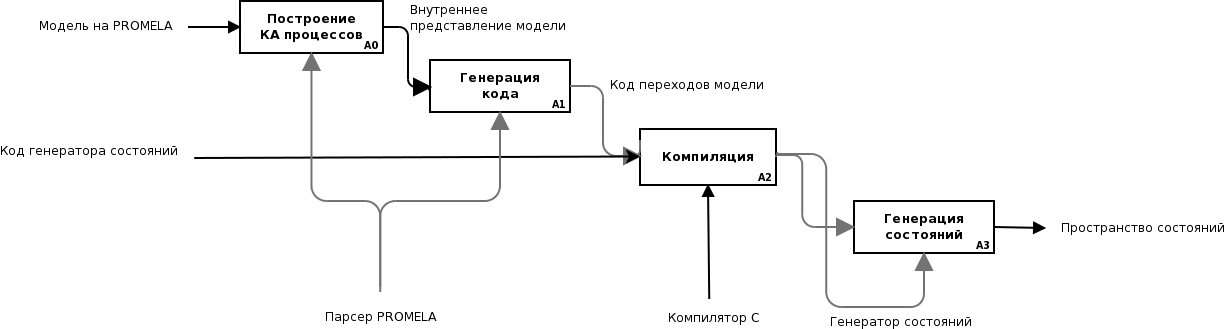
\includegraphics[width=1\textwidth]{../graphics/idef0-codegen}  
  \caption{Схема процесса верификации}
\label{fig:idef0-codegen}
\end{figure}

Генерируемый код на~C проверяет условия выполнимости текущих инструкций всех процессов и,
в случае выполнимости процесса $P$, создает новое состояние, являющееся копией текущего, и
модифирует его в соответствии с текущей инструкцией $P$.

Таким образом, генерируются следующие части кода:

\begin{itemize}
\item проверка выполнимости процессов данного состояний;
\item модификация состояния в соответствии с текущей инструкцией данного процесса;
\item вспомогательный код (отладочная печать состояния и т.п.).
\end{itemize}

Полученный код компилируется и компонуется вместе вместе с программой-<<драйвером>>
(осуществляющей выполнение не зависящих от конкретной модели операций: хэширование и
хранение состояний, передача по сети и~т.д.). Программа-<<драйвер>> делает вызовы функций
сгенерированного кода для вычисления $Next(s)$.

<<Драйверов>> имеется два: 

\begin{itemize}
\item последовательный, использованный в \ref{cha:paremu} для имитации параллельного
  выполнения с целью оценки распредления состояний;
\item описанный в \ref{cha:parmpi} параллельный на MPI.
\end{itemize}

\section{Генератор кода}
\label{sec:promela-parser}

Парсер описания модели и генератор кода написан на языке Python. В качестве парсера
используется штатный GLR-парсер \Code{Pyggy}. Диаграмма классов генератора показана на
рис.~\ref{fig:pmlparse-classes}.

\begin{figure}[ht]
  \centering
  \includegraphics[width=1\textwidth]{../graphics/pmlparse-classes}
  \caption{Диаграмма классов генератора кода}
  \label{fig:pmlparse-classes}
\end{figure}

% \section{Тестирование основных модулей программного комплекса}
% В данном разделе приводится описание результатов модульного тестирования программного комплекса. Тестируется 
% вспомогательный функционал, не участвующий непосредственно в процессе верификации.

% \textbf{Загрузка конфигурационных файлов}

% Классы эквивалентности для действия "Загрузка конфигурационных файлов" приведены в табл. 
% \ref{tab:equclass_conf_load}.

% \begin{table}[!ht]
%   	\caption{Классы эквивалентности для действия "Загрузка конфигурационных данных"}
% 	\begin{tabular}{|p{8cm}|p{8cm}|}
% 		\hline
% 			Допустимые классы эквивалентности & Недопустимые классы эквивалентности \\
% 		\hline
% 			Все существующие и синтаксически корректные YAML-файлы & Некорректные YAML-файлы; несуществующие файлы \\
% 		\hline
% 	\end{tabular}
% 	\label{tab:equclass_conf_load}
% \end{table}

% Описания тестов для данного действия приведены в табл. \ref{tab:testcase_conf_load}.
% \begin{table}[!ht]
%   	\caption{Тестовые случаи для действия "Загрузка конфигурационных данных"}
% 		\begin{tabular}{|p{4cm}|p{4cm}|p{3cm}|p{3cm}|}
% 			\hline
% 			Описание & Входные данные & Ожидаемый результат & Полученный результат \\
% 			\hline
% 			Несуществующий файл& "" & Сообщение "Файл не существует" & Сообщение "Файл не существует" \\
% 			\hline
% 			Пустой файл& "" & Корректный файл & Корректный файл\\
% 			\hline
% 			Файл с некорректной табуляцией& "vars:$\backslash$n$\backslash$ta:$\backslash$n $\backslash$ttype: 'double'" & Сообщение "Ошибка в строке 3" & Сообщение "Ошибка в строке 3"\\
% 			\hline
% 			Корректный заполненный файл& "vars:$\backslash$n$\backslash$ta:$\backslash$n $\backslash$t$\backslash$ttype: 'double' & Корректный файл & Корректный файл\\
% 			\hline
% 	\end{tabular}
% 	\label{tab:testcase_conf_load}
% \end{table}

% \textbf{Проверка структуры модели}

% Классы эквивалентности для действия "Проверка структуры модели" приведены в табл. 
% \ref{tab:equclass_conf}.

% \begin{table}[!ht]
%   	\caption{Классы эквивалентности для действия "Проверка структуры модели"}
% 	\begin{tabular}{|p{8cm}|p{8cm}|}
% 		\hline
% 		Допустимые классы эквивалентности & Недопустимые классы эквивалентности \\
% 		\hline
% 		Корректно описанные модели (в соответствии с разделом 3.2) & Некорректно описанные модели \\
% 		\hline
% 	\end{tabular}
% 	\label{tab:equclass_conf}
% \end{table}

% Описания тестов для данного действия приведены в табл. \ref{tab:testcase_conf}.

% \begin{table}[!ht]
%   	\caption{Тестовые случаи для действия "Проверка структуры модели"}
% 	\begin{tabular}{|p{5cm}|p{5cm}|p{5cm}|}
% 		\hline
% 		Описание & Ожидаемый результат & Полученный результат \\
% 		\hline
% 		Модель без секции с описанием состояний & 
% 		Сообщение "Наличие описания состояний обязательно" & 
% 		Сообщение "Наличие описания состояний обязательно" \\
% 		\hline
% 		Модель без секции с описанием входных данных &
% 		Сообщение "Наличие описания входов обязательно" &  
% 		Сообщение "Наличие описания входов обязательно"\\
% 		\hline
% 		Вероятности переходов для одного из состояний имеет сумму, б\textit{о}льшую 1 & 
% 		Сообщение "Сумма указанных вероятностей не должна превышать 1" &
% 		Сообщение "Сумма указанных вероятностей не должна превышать 1"\\
% 		\hline
% 		Корректная модель & 
% 		Проверка пройдена &
% 		Проверка пройдена \\
% 		\hline		
% 	\end{tabular}
% 	\label{tab:testcase_conf}
% \end{table}

% \textbf{Проверка параметров командной строки}

% Классы эквивалентности для действия "Проверка параметров командной строки" приведены в табл. 
% \ref{tab:equclass_console}.

% \begin{table}[!ht]
%   	\caption{Классы эквивалентности для действия "Проверка структуры модели"}
% 	\begin{tabular}{|p{8cm}|p{8cm}|}
% 		\hline
% 		Допустимые классы эквивалентности & Недопустимые классы эквивалентности \\
% 		\hline
% 		Корректные параметры (в соответствии с разделом 3.6) & Некорректные параметры \\
% 		\hline
% 	\end{tabular}
% 	\label{tab:equclass_console}
% \end{table}

% Описания тестов для данного действия приведены в табл. \ref{tab:testcase_console}.

% \begin{table}[!ht]
%   	\caption{Тестовые случаи для действия "Проверка структуры модели"}
% 	\begin{tabular}{|p{4cm}|p{4cm}|p{3cm}|p{3cm}|}
% 		\hline
% 		Описание & Входные данные & Ожидаемый результат & Полученный результат \\
% 		\hline
% 		Недопустимый параметр &
% 		"-u 170" &
% 		Сообщение "Недопустимый параметр: u" & 
% 		Сообщение "Недопустимый параметр: u" \\
% 		\hline
% 		Недопустимое значени &
% 		"-cway z" &
% 		Сообщение "Параметр cway имеет недопустимое значени: z" &  
% 		Сообщение "Параметр cway имеет недопустимое значени: z"\\
% 		\hline
% 		Вызов без параметров & 
% 		"" &
% 		Корректное поведение (берутся значения по умолчанию) &
% 		Корректное поведение (берутся значения по умолчанию)\\
% 		\hline
% 		Вызов с одним параметром & 
% 		"-r" &
% 		При генерации наборов используется только случайный метод&
% 		При генерации наборов используется только случайный метод \\
% 		\hline		
% 	\end{tabular}
% 	\label{tab:testcase_console}
% \end{table}

%% USE CASE
% В процессе анализа предметной области и поставленных задач выявлены следующие прецеденты, 
% показанные на рис. \ref{use_case}:

% \begin{itemize}
% \item подготовка исходной модели;
% \item управления параметрами верификации;
% \item проведение верификации;
% \item выдача результатов.
% \end{itemize}

% \subsection{Подготовка исходной модели}
% Прецедент служит для создания и модификации моделей: добавление, изменение и удаление информации в текстовом 
% режиме.

% Предусловия: нет.

% \textit{Основной сценарий.} 

% \begin{enumerate}
% \item Пользователь формирует конфигурационный файл в соответствии с требованиями к его составу.
% \item Пользователь указывает программе путь к конфигурационному файлу.
% \item Программа загружает и обрабатывает файл.
% \item Программа выдает сообщение об успешной обработке файла.
% \end{enumerate}

% \textit{Альтернативный сценарий 1.}
% \begin{enumerate}
% \item Пользователь формирует конфигурационный файл в соответствии с требованиями к его составу.
% \item Пользователь указывает программе путь к конфигурационному файлу.
% \item Программа не обнаруживает файл по указанному пути, так как он не верен.
% \item Программа выдает сообщение об ошибке "Некорректный путь к файлу".
% \end{enumerate}

% \textit{Альтернативный сценарий 2.}
% \begin{enumerate}
% \item Пользователь формирует конфигурационный файл в соответствии с требованиями к его составу.
% \item Пользователь указывает программе путь к конфигурационному файлу.
% \item Программа загружает и обрабатывает файл.
% \item Программа обнаруживает синтаксическую ошибку в структуре файла.
% \item Программа выдает сообщение об ошибке "Синтаксическая ошибка" с указанием строки, содержащей ошибку.
% \end{enumerate}

% \textit{Альтернативный сценарий 3.}
% \begin{enumerate}
% \item Пользователь формирует конфигурационный файл в соответствии с требованиями к его составу.
% \item Пользователь указывает программе путь к конфигурационному файлу.
% \item Программа загружает и обрабатывает файл.
% \item Программа обнаруживает семантическую ошибку (не описаны обязательные блоки) в структуре файла.
% \item Программа выдает сообщение об ошибке "Не описан блок" с указанием требуемого блока.
% \end{enumerate}

%%% Local Variables: 
%%% mode: latex
%%% TeX-master: "main"
%%% End: 
